% upLaTeX文書
% \documentclass[uplatex,a4paper]{jsarticle}
\documentclass[pdflatex,ja=standard]{bxjsarticle}
% デフォルトのフォント設定のまま!
\usepackage{color}
\usepackage{url}
\usepackage{graphicx}
\usepackage{algorithm}
\usepackage{algorithmic}

\definecolor{myred}{rgb}{0.85,0,0.1}
\definecolor{mypink}{rgb}{1,0.92,0.92}
\setlength{\fboxsep}{2pt}


\title{情報メディア演習B-2 授業レポート}
\author{201821636 1班 村松直哉}
\date{\today}
\begin{document}
\maketitle
%
%
\section{テーマ}
我々は本ワークショップのテーマとして,「図書館 $x$ エロ」と設定した.

「エロ」という概念は,人間と切り離せないものであり,経済的にも大きな影響力がある.
つまり,ワークショップの参加者全員が興味を持つことができ,かつ非常に重要なテーマであると言える.


\section{KJ法の結果} \label{sec:kj}
授業中に行ったKJ法の結果を図\ref{fig:result}に示す.
チームメンバーから出たアイディアをまとめて,図のようにまとめた.

\begin{figure}[htb]
\begin{center}
    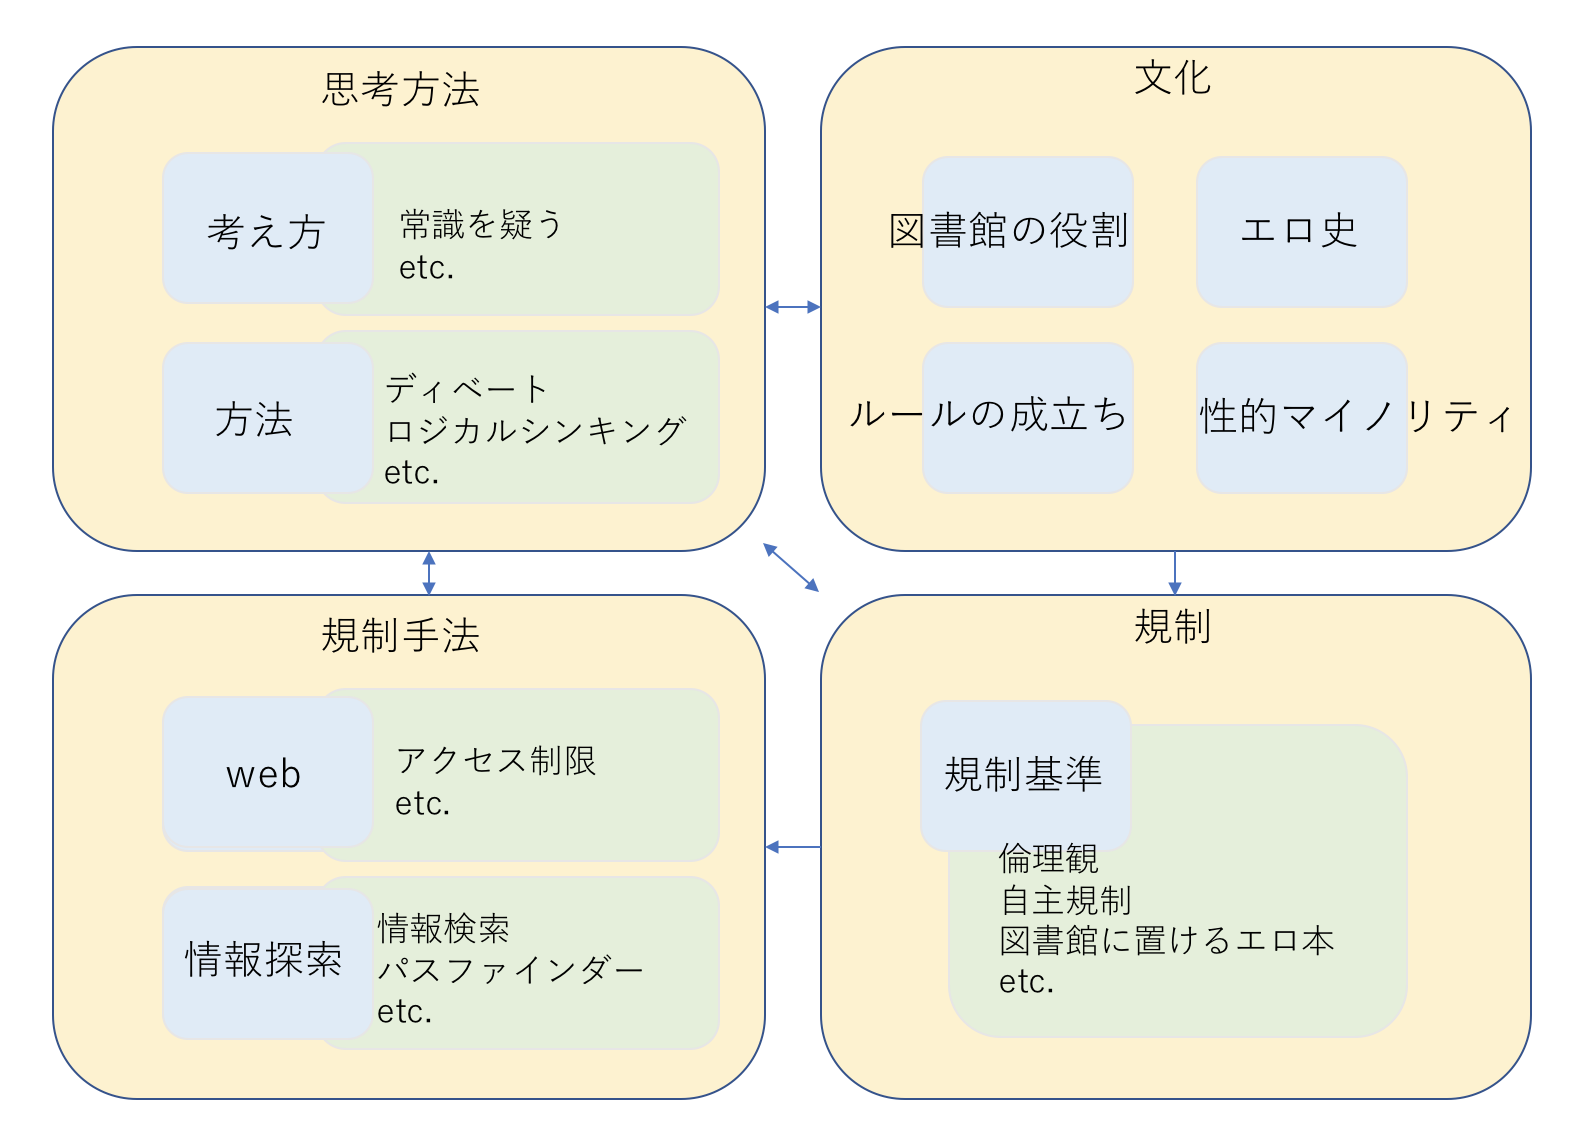
\includegraphics[width=14cm]{figs/result.png}
\end{center}
\caption{KJ法による分類結果}
\label{fig:result}
\end{figure}


\section{ワークショップのアイディア}
\ref{sec:kj}から出たアイディアでは,大きなテーマとして「思考方法」が全ての大テーマと繋がっている.
そのため,「思考方法」を元にアイディアをまとめ,ワークショップの目的として,以下のようなものをあげた.
\begin{itemize}
    \item 課題から逆算して考える論理的思考を学ぶ
    \item 図書館について深く考える
\end{itemize}

この目標を達成するために,「ディベート」と「資料作成」の2つの要素を取り入れることを考えた.
これらの要素の重要性を解説し,ワークショップの概要に付いて以下の章で述べる.

\subsection{ディベート}
ディベートは勝ち負けがあり,そのために対象の事柄について深く理解する必要がある.
また,「エロ」という社会的に重要なテーマを扱っているため,議論が活発になることが容易に予想される.
これにより,ワークショップ全体が,大いに盛り上がる.

ディベートは,相手チームの主張内容を予測し,事前に回答を作ることが必要とされる.
これにより,どちらのチームに所属したとしても,両方の意見について,自ら深く考えることができる.
ディベートを通して,ワークショップの目的の一つである「図書館について深く考える」ことができる.

\subsection{資料作成}
ディベートを行う際に,各チームはそれぞれ,資料を作成する必要がある.
そして,その資料は審判を説得するために,情報が分かりやすくまとまっていることが求められる.
これはまさに論理的思考によって作られるものである.

また資料作成は,大学入学後に授業などで頻繁に求められるため,大学について理解を深めたい,高校生にとっても非常に有用である.

\subsection{ワークショップの概要}
私が提案する討論型ワークショップの手順を以下に示す.
\begin{itemize}
    \item 1日目
    \begin{enumerate}
        \item 男女のヌードを描いた様々な書籍を集める.
        \item 参加者はそれぞれ自分の考えで,図書館に所蔵するべきか否かを投票する.
        \item ワークショップ参加者の意見が最も割れた書籍を,討論対象書籍とする.
        \item 参加者は,それぞれの意見の2チームに別れる.
        \item 論理的思考の講義を行う.
        \item 一定時間,チーム内で意見をまとめ,それに従ってディベートのための資料を作る.
    \end{enumerate}
    \item 2日目
    \begin{enumerate}
        \item 教員を審判として,両チームでディベートを行う.
        \item ディベートの振り返りと反省を両チームで行う.
        \item 反省を両チームで発表し合う.
        \item 教員から実際の図書館の性教育図書に関する現状を講義形式で伝える.
    \end{enumerate}
\end{itemize}

世界的に日本の性教育は,非常に遅れている.
それにより,性に対する偏った考え方ばかりが,広まる傾向にあることが懸念されている.
性については,誰もが直面する課題であるにも関わらず,文化的な背景から,性について真剣に考える場は多くない.

そこで本学類のメイントピックである「図書館」に対して,性やいわゆる「エロ」を扱った図書について議論させる.
これにより,図書館の理解が深まるだけでなく,性に関する知識や考え方も深まり,高校2年生という成長過程における重要な時期において,楽しく知識を深められることを期待している.


\section{他グループからの提案}
他グループからの意見を以下にまとめる.
ただし,$x$は読解できなかった文字を示している.
また,それぞれの意見の特性に合わせて,分類を行っている.

\begin{itemize}
    \item 肯定的
    \begin{itemize}
        \item 面白い発想の構造図
        \item エロかった.分類は良かった.
        \item エロを分析した結果,何を得るのか明確にするといいと思う.
        \item シャープでしょ.
        \item 一番見やすい構造だった.ワークショップもよく考えられている.
        \item ワークショップを全体として考えるのでなく,ワークショップを流れの一部としている点が良かったです.
    \end{itemize}
    \item 問題提起
    \begin{itemize}
        \item 高校生にエロ本を持ち寄らせる発想はユニークだが,エロを全面的にプッシュすると参加者層の偏りがありそう.ある程度,真面目な人が参加するには...?
        \item 高校2年生... 17才.18禁的な話が難しそう.
        \item 青の枠線に違う小テーマが入っており,黄色と緑の付箋が混ぜているため,わかりにくくなります.
        \item 斬新なテーマについて深く掘り下げられていてすごく興味深いと思いました.ただ思春期真っ盛りの高校生には刺激的すぎるテーマかも.
    \end{itemize}
    \item 提案
    \begin{itemize}
        \item 図\ref{fig:propose}みたいな構造の方が良い.
        \item 流れがわかるように時系列で示したら良いかもしれない.
        \item 先ずは文化があるという構造な,「文化」が一番大きな枠な構造でもよかったかも.
    \end{itemize}
    \item 不明
    \begin{itemize}
        \item 図書館を言及した中分類が$x$いとういう印象を受けた.
    \end{itemize}
\end{itemize}

肯定的な意見が半分近くあり,ある程度の理解を得られたことがわかる.
「問題提起」や「提案」には,非常に有用な意見が多くあった.

問題提起には,高校生に対して,刺激的な内容でワークショップを行うことに対する懸念が目立つ.
これについては,日本の性教育問題と関係しており,ユネスコのガイダンスは5歳児からとある~\cite{40021294461}.
そのため高校2年生は,性に関する話題を扱うのに十分に成熟した年齢であると考える.

その他の意見として,分類した構造に問題があることや,改善案が多く示された.
「文化」という大きなテーマで囲っても良い.
しかし,これは「文化」という言葉自体が大きな概念過ぎるため,分類した時の用語として不適切だったと考えられる.
別の意見としてあった,ワークショップの流れとして,時系列順に並べるという提案は,良いまとめ方である.

\begin{figure}[htb]
\begin{center}
    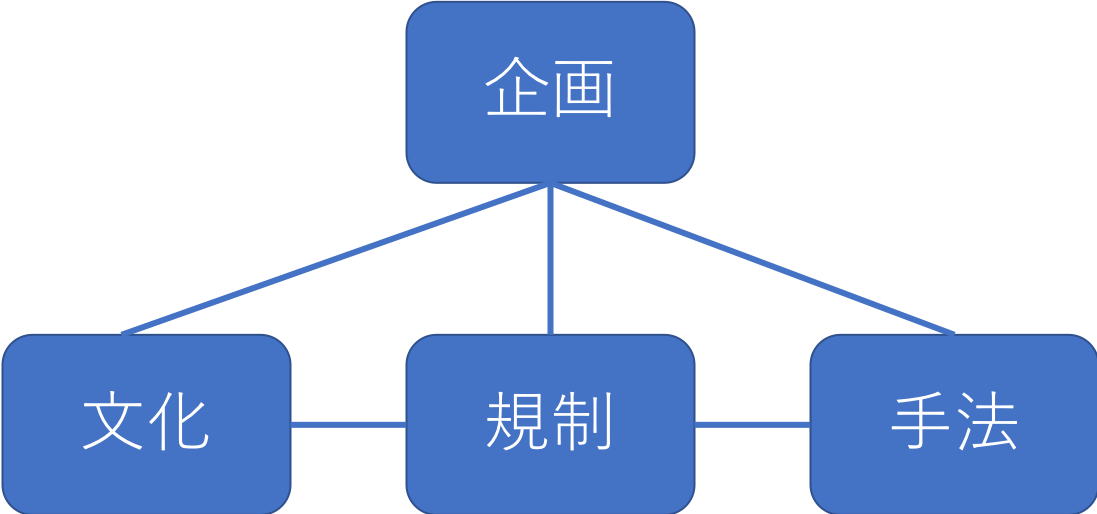
\includegraphics[width=14cm]{figs/propose.png}
\end{center}
\caption{KJ法による分類結果}
\label{fig:propose}
\end{figure}


\bibliographystyle{ieee}
\bibliography{references}

\end{document}
